\chapter{Practical Information}


\section{Conference Venue}
MCM 2025 is hosted by Illinois Institute of Technology (Illinois Tech).  All talks will take place on the Mies Campus in the following three buildings
\begin{itemize}
	\item Hermann Hall (HH),
	\item Perlstein Hall (PH), and
	\item Wishnick Hall(WH)
\end{itemize}
See the campus map on the next page or at \href{https://www.iit.edu/sites/default/files/2022-08/mies-campus-accessibility-map-2022.pdf}{this link}.  

The registration desk, the coffee breaks, and the Monday night welcome reception will all be  in the Hermann Hall Lobby.

\clearpage

\begin{center}
	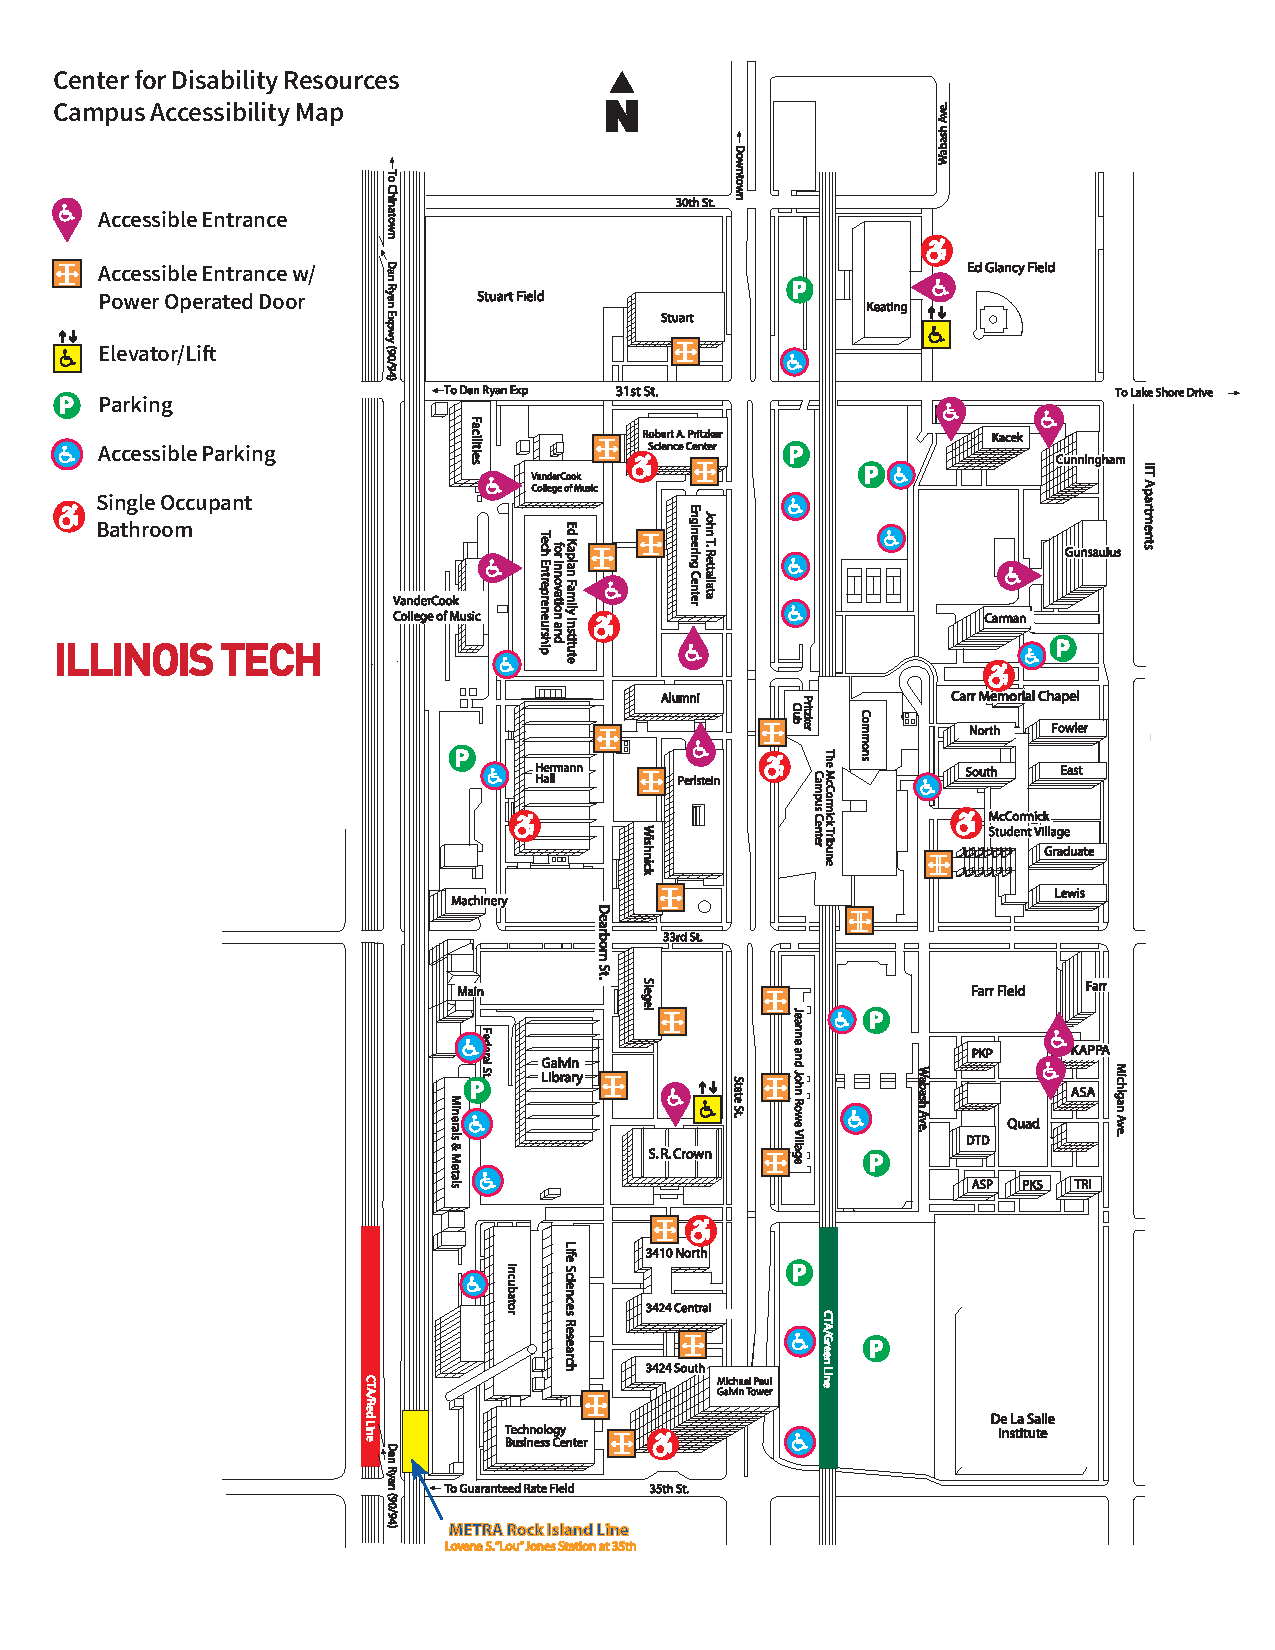
\includegraphics[width = \textwidth] {Photos/mies-campus-accessibility-map-2022.pdf}
\end{center}



\begin{center}
	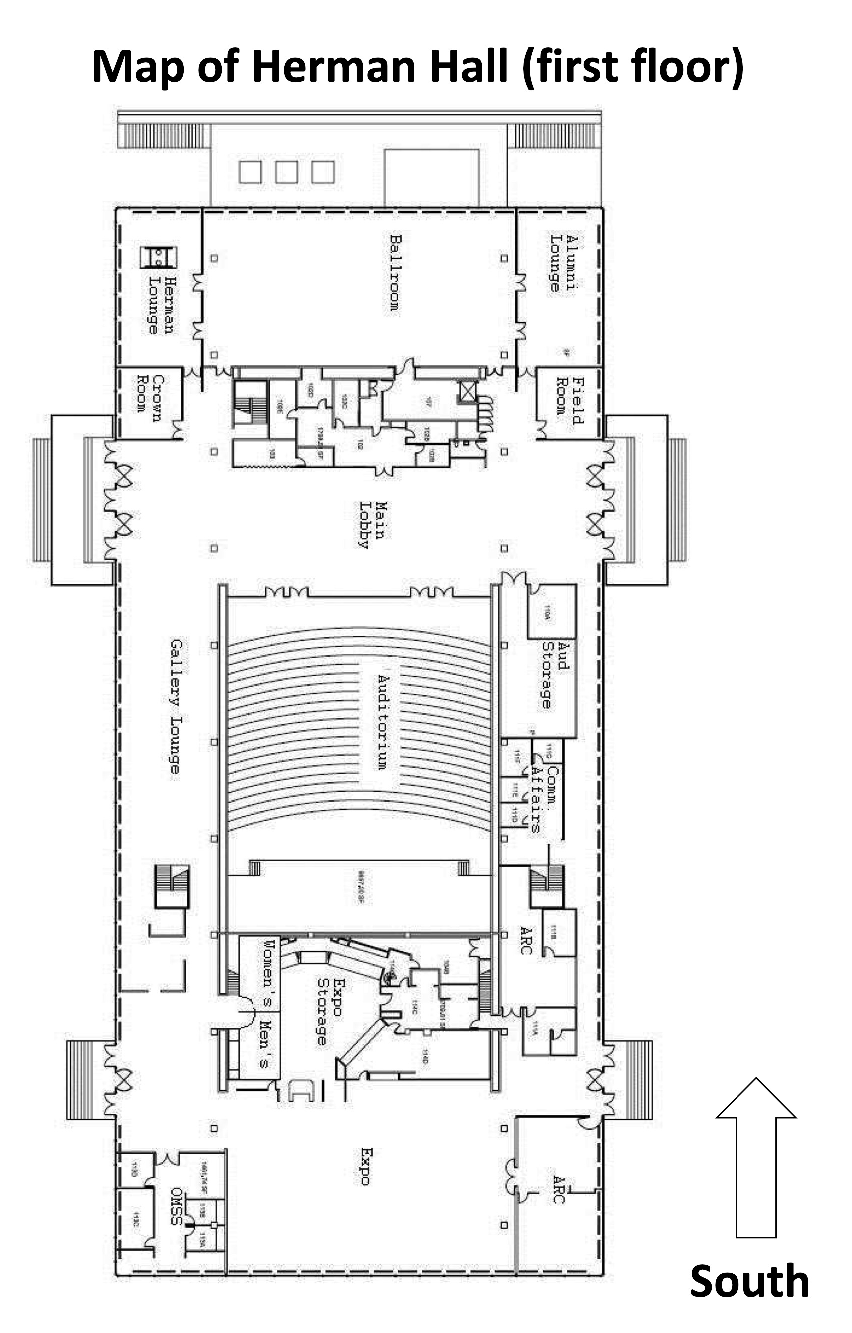
\includegraphics[width =0.95 \textwidth] {Photos/MapHermannHallFirstFloor_cropped.eps}
\end{center}
\clearpage

\section{Getting to Illinois Tech}

\subsection{Local Transportation}
Illinois Tech is located several miles south of downtown.  You  can reach Illinois Tech via 
\begin{itemize}
	\item the Chicago Transit Authority (\href{https://www.transitchicago.com/schedules/}{CTA}) `L' Green or Red Lines, which stop at 35th Street, 
	\item the href{https://www.transitchicago.com/schedules/}{CTA} Route 29 bus, which stops at the corner of State and 32nd Streets, or
	\item taxi, Uber, or Lyft.
	 \item If you are driving to Illinois Tech, there is paid visitor parking in the lot on the east side of State Street between 31st and 32nd Streets (enter via State Street).
\end{itemize}

\subsection{Getting to Chicago}

\begin{itemize}
  \item Two major airports, \href{https://www.flychicago.com/ohare/home/Pages/default.aspx}{O'Hare} and \href{https://www.flychicago.com/midway/pages/default.aspx}{Midway} serve Chicago, and are not far from Illinois Tech.  
  \item Our main domestic passenger rail line is \href{Amtrak}{https://www.amtrak.com/home.html}.
\end{itemize}


\section{Food}

Meals will \emph{not} be provided, except for the Wednesday night conference banquet. There are several places on campus or nearby where you can purchase meals.  They are show in \href{https://www.google.com/maps/d/u/1/edit?mid=1QH5guZDg-m8_f1oO9HgZ5sIL76q1gdk&usp=sharing}{this Google map}


\begin{itemize}
	\item Cafeteria in the McCormick Tribune Conference Center near State and 32nd Street
	\item On 31st Street between Near W
	\begin{itemize}
		\item \href{https://www.yelp.com/biz/yees-cantonese-kitchen-chicago-2?osq=Restaurants} {Yee's Cantonese Kitchen}  
	\end{itemize}
		\item Near the corner of 33rd Street and Wentworth Avenue Streets
	\begin{itemize}
		\item Jimmy John's submarine sandwiches
		\item Starbucks
	\end{itemize}
	
	\item Near the corner of 35th and State Streets
	\begin{itemize}
		\item Jimmy John's submarine sandwiches
		\item Starbucks
	\end{itemize}


\end{itemize}



%\begin{center}
% \includegraphics[width=14cm]{Food_map}
%\end{center}


\section{Technology}

\subsubsection{Equipment in classrooms used for conference}

TBD


\subsubsection{Internet Access}

Illinois Institute of Technology is a partner with eduroam, and you can get internet access via that route if your institution is an eduroam partner.

[IIT guests to be filled in]

\subsubsection{Electrical Power}

In the United States, the standard voltage is 120V at a frequency of 60Hz.  The standard power plugs are 
\begin{itemize}
	\item Type A (two flat parallel pins) and 
	\item Type B (two flat parallel pins plus a round grounding pin).
\end{itemize}

\section{Health and Safety}

This conference adheres to the nondiscrimination policies of the Illinois Institute of Technology  and also of the University of Chicago (see \href{https://www.uchicago.edu/non-discrimination){\nolinkurl{www.uchicago.edu/non-discrimination]}, which houses our sponsor the US NSF Institute for Mathematical and Statistical innovation(IMSI).


\subsubsection{Emergency Contacts, Hospitals and Services on Campus}

TBD



\section{Conference Statistics (as of \today)}

\begin{center}
 \begin{tabular}{ll}
 Number of participants & ?? \\
 Number of plenary lectures & 8 \\
 Number of talks & ?? \\
 Number of special sessions & ?? \\
 Number of technical sessions & ?? \\
 \end{tabular}
\end{center}